\begin{figure}
    \centering
    \begin{subfigure}{\linewidth}
    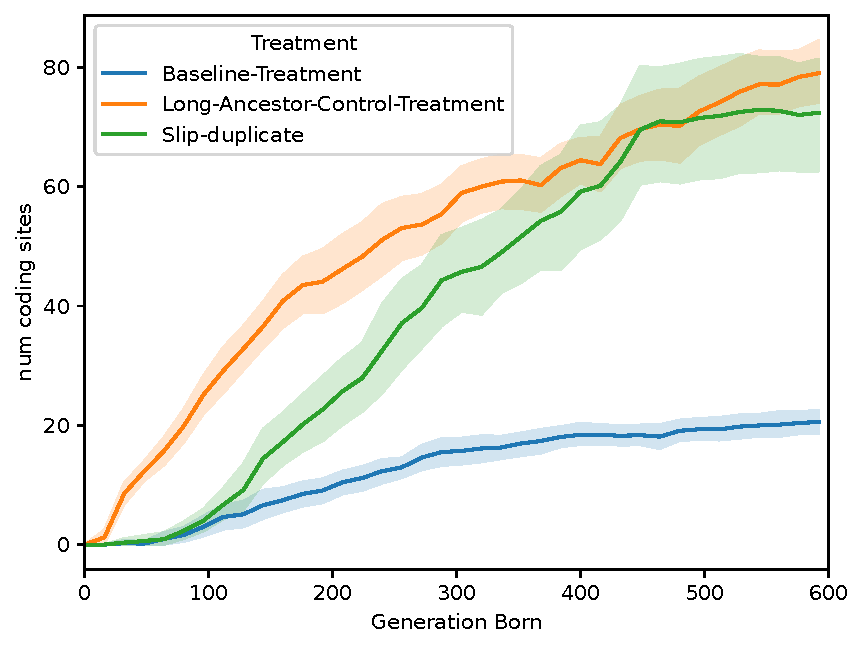
\includegraphics[width=\linewidth]{binder/binder/teeplots/hue=treatment+post=plt-xlim-0-600+viz=lineplot+x=generation-born+y=num-coding-sites+ext=.pdf}
    \caption{\footnotesize number coding sites (critical for tasks)}
    \label{fig:num-coding-sites:coding}
    \end{subfigure}

    \begin{subfigure}{\linewidth}
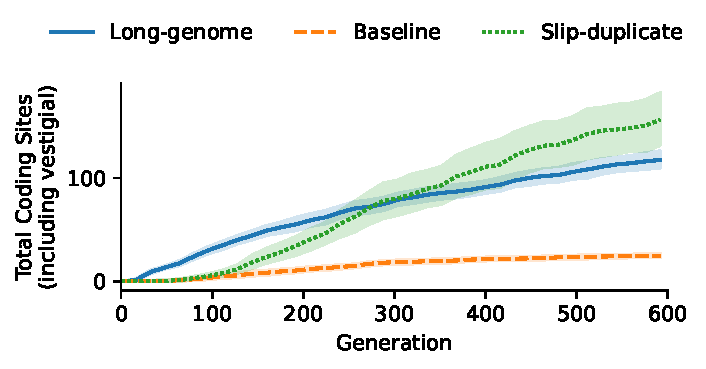
\includegraphics[width=\linewidth,clip, trim=0 0 0 0.8cm]{binder/binder/teeplots/hue=treatment+post=plt-xlim-0-600+viz=lineplot+x=generation-born+y=num-coded-sites+ext=.pdf}
    \caption{\footnotesize number of sites that currently or have coded for a task}
    \label{fig:num-coding-sites:coded}
    \end{subfigure}
    \caption{
        \textbf{Growth trajectories of brittleness and coding site counts over evolutionary time.}
        \footnotesize
        Error bands give 95\% CI, bootstrapped over 30 replicates per treatment.
    }
    \label{fig:num-coding-sites}
\end{figure}
